\chapter{Advanced model order reduction techniques for PDE-constrained optimization}
In \cite{KV99}, POd has been applied to obtain a reduced model of Burgers' equation...
\begin{equation}
\label{allgControl_small}
\begin{split}
\min_{u} \ &\tilde{\mathcal{J}}(\tilde{y},u) ,\\
\text{subject to } \ &\tilde{c}(\tilde{y},u) = 0,
\end{split}
\end{equation}
Similarly, we denote $\hat{\tilde{\mathcal J}}(u) := \tilde{\mathcal{J}}(\tilde{y}(u),u)$.
\section{A POD-DEIM reduced model for optimal control of Burgers' equation}
\label{redOptimalControl}
%In Section \ref{fullOrderControl}, the full-order optimization problem \eqref{minJ}-\eqref{Burgers2} has been discretized and solved numerically by the Newton-CG method and Armijo line-search as proposed in \cite{H08}. We now want to apply POD-DEIM in order to derive a reduced optimization problem. Therefore, we introduce the reduced state and control variables $\mathbf{\tilde y}(t)$ and $\mathbf{\tilde u}(t)$  via,
%\begin{align}
%\label{approx_yu1}
%\mathbf{y}(t) &\approx \Phi_\ell \mathbf{\tilde y}(t), \quad \mathbf{\tilde y} \in \mathbb{R}^\ell, \\
%\label{approx_yu2}
%\mathbf{u}(t) &\approx \Psi_\ell \mathbf{\tilde u}(t), \quad \mathbf{\tilde u} \in \mathbb{R}^\ell,
%\end{align}
%where $\Phi_\ell$ is computed as described in \eqref{Phidef}, and $\Psi_\ell$ is a matrix that contains the principle components of the full-order control $\mathbf{u}(t)$. We obtain $\Psi_\ell$ from the left singular vectors of the snapshot matrix $U := [\mathbf{u}(t_1),...,\mathbf{u}(t_{n_s})]$, i.e.
%\begin{align}
%\label{Psidef}
%U = \Psi \Sigma V^T,
%\end{align}
%where $\Psi_\ell$ consists of the first $\ell$ columns of $\Psi$ and $\Sigma, V$ are unused.

%If we plug-in the approximations \eqref{approx_yu1}-\eqref{approx_yu2} into the full-order cost functional \eqref{minJ_discr}, the reduced cost functional is given by,
\begin{align}
\label{redOpt}
\min_{\mathbf{u}_0,...,\mathbf{u}_{N_t}} \tilde{J}(\mathbf{\tilde y}_0,...,\mathbf{\tilde y}_{N_t},\mathbf{u}_0,...,\mathbf{u}_{N_t}) = \min_{\mathbf{u}_1,...,\mathbf{u}_{N_t}} \sum_{i=0}^{N_t} \delta \! t \left( \frac{1}{2} \mathbf{\tilde y}_i^T \mathbf{\tilde y}_i - \mathbf{\tilde z}^T\mathbf{\tilde y}_i + \frac{\omega}{2}\mathbf{u}_i^T M \mathbf{u}_i \right),
\end{align}
where the reduced desired state is,
\begin{align}
\label{zred}
\mathbf{\tilde z} &:= \Phi_\ell^T \mathbf{z} \in \mathbb{R}^\ell,\\
%\label{M2red}
%\tilde M &:= \Psi_\ell^T M \Psi_\ell \in \mathbb{R}^{\ell \times \ell}.
\end{align}
Note that both only depend on the small dimension $\ell$.

In order to obtain a POD-DEIM reduced model for the constraining Burgers' equation, we refer to Section \ref{fullOrderControl} and apply the POD-DEIM projection to \eqref{Burgers2_discr}. The fully discretized reduced constraint is, thus, given by
\begin{align}
\label{redBurgers}
\tilde{c}_i(\mathbf{\tilde y}_i,\mathbf{\tilde y}_{i+1},\mathbf{\tilde u}_{i+1}) \equiv \frac{1}{\delta \! t} \mathbf{\tilde y}_{i+1} - \frac{1}{\delta \! t}\mathbf{\tilde y}_i + \frac{1}{2} \tilde{B}(\tilde{F}\mathbf{\tilde y}_{i+1})^2 + \nu \tilde{C}\mathbf{\tilde y}_{i+1} - \mathbf{\tilde f} - \tilde{\tilde{M}}\mathbf{\tilde u}_{i+1} = 0, \quad i=0,...,N_t-1,
\end{align}
where
\begin{align}
\label{fred}
\mathbf{\tilde f} &:= \Phi_\ell^T \mathbf{f} \in \mathbb{R}^\ell,\\
\label{M1red}
\tilde{\tilde{M}} &:= \Phi_\ell^T M \Psi_\ell \in \mathbb{R}^{\ell \times \ell},
\end{align}
and $\tilde{B}, \tilde{C}, \tilde{F}$ are defined in \eqref{Bred}, \eqref{Cred}, \eqref{Fred}, respectively.

Note, that the nonlinear term in \eqref{redBurgers} has to be considered as a function of the reduced variable $\mathbf{y}$ and has the slightly more complicated form,
\begin{align}
 \label{redNonlin}
 \tilde{\mathcal{N}}(\mathbf{\tilde{y}}_{i+1}) := \frac{1}{2} \tilde{B} (\tilde{F} \mathbf{\tilde{y}}_{i+1})^2.
\end{align}

The Lagrangian function of the reduced model can be obtained directly from \eqref{redOpt} and \eqref{redBurgers} and is given by,
\begin{align}
\label{redLag}
&\mathcal{\tilde L}(\mathbf{\tilde y}_0,...,\mathbf{\tilde y}_{N_t}, \mathbf{\tilde u}_0,...,\mathbf{\tilde u}_{N_t},\boldsymbol{\tilde \lambda}_1,...,\boldsymbol{\tilde \lambda}_{N_t}) \nonumber \\
&\ = \sum_{i=0}^{N_t} \delta \! t \left( \frac{1}{2} \mathbf{\tilde y}_i^T \mathbf{\tilde y}_i - \mathbf{\tilde z}^T\mathbf{\tilde y}_i + \frac{\omega}{2} \mathbf{\tilde u}_i^T \tilde{M} \mathbf{\tilde u}_i \right) \nonumber \\
&\quad +  \sum_{i=0}^{N_t-1} \boldsymbol{\tilde \lambda}_{i+1}^T \left( \frac{1}{\delta \! t} \mathbf{\tilde y}_{i+1} - \frac{1}{\delta \! t} \mathbf{\tilde y}_i + \frac{1}{2} \tilde{B} (\tilde{F} \mathbf{\tilde y}_{i+1})^2 + \nu \tilde{C} \mathbf{\tilde y}_{i+1} - \mathbf{\tilde f} - \tilde{\tilde{M}} \mathbf{\tilde u}_{i+1}  \right)
\end{align}
Note, that even $\boldsymbol{\tilde \lambda}_i \in \mathbb{R}^\ell$. If we choose $k = \ell$, then \eqref{redLag} only depends on $\ell$.

\section{A Newton-type method for the POD-DEIM reduced model}
\label{Newton_red_chapter}
\begin{algorithm}[H]
\caption{Algorithm \ref{alg:Adj1} applied to the reduced Burgers' model}
\label{alg:Adj1_redBurgers}
\begin{algorithmic}[1]
\STATE From the initial condition $\mathbf{\tilde y}_0$ and the current control $\mathbf{\tilde u}_0,...,\mathbf{\tilde u}_{N_t}$, solve the reduced Burgers' equation for $\mathbf{\tilde y}_1,...,\mathbf{\tilde y}_{N_t}$ as described in Section \ref{BurgersPODDEIM}
\STATE The adjoint equation \eqref{adjoint1} reads:
\begin{subequations}
\begin{align}
\label{AdjRedOrder_term}
\left(\frac{1}{\delta \! t}I_\ell + \tilde{\mathcal{N}}'(\mathbf{\tilde{y}}_{N_t})  +  \nu \tilde{C}\right)^T \boldsymbol{\tilde{\lambda}}_{N_t} &= -\delta \! t(\mathbf{\tilde{y}}_{N_t} - \mathbf{\tilde z} )\\
\label{AdjRedOrder}
\left(\frac{1}{\delta \! t}I_\ell + \tilde{\mathcal{N}}'(\mathbf{\tilde{y}}_{i})  + \nu \tilde{C}\right)^T \boldsymbol{\tilde{\lambda}}_i &= - (-\frac{1}{\delta \! t} I_\ell)^T \boldsymbol{\tilde{\lambda}}_{i+1} -\delta \! t( \mathbf{\tilde{y}}_{i} - \mathbf{\tilde z} ), \quad i = N_t-1,...,1
\end{align}
\end{subequations}
\STATE The gradient is computed according to formula \eqref{grad}:
\begin{align}
\label{gradRedOrder}
\nabla_{\tilde u} \hat{\tilde{\mathcal J}}(\mathbf{\tilde{u}}_0,...,\mathbf{\tilde{u}}_{N_t}) = \begin{pmatrix} \delta \! t \omega \tilde{M} \mathbf{\tilde{u}}_0 \\ \delta \! t \omega \tilde{M} \mathbf{\tilde{u}}_1 - \tilde{\tilde{M}}^T \boldsymbol{\tilde{\lambda}}_1 \\ \vdots \\ \delta \! t \omega \tilde{M} \mathbf{\tilde{u}}_{N_t} - \tilde{\tilde{M}}^T \boldsymbol{\tilde{\lambda}}_{N_t} \end{pmatrix}
\end{align}
\end{algorithmic}
\end{algorithm}
Here, $I_\ell$ is the $\ell \times \ell$ identity matrix and,
\begin{align*}
\tilde{\mathcal{N}}'(\mathbf{\tilde{y}}) = \frac{d}{d \mathbf{\tilde{y}}} \left( \frac{1}{2} \tilde{B} (\tilde{F}\mathbf{\tilde{y}})^2 \right) = \begin{pmatrix} \tilde{B}_{1,1} & \hdots & \tilde{B}_{1,m}\\ \vdots & & \vdots \\ \tilde{B}_{\ell,1} & \hdots & \tilde{B}_{\ell,m}  \end{pmatrix} \cdot \begin{pmatrix} \mathbf{\langle \tilde{y}} , \tilde{F}_1\rangle \tilde{F}_{1,1} & \hdots & \langle \mathbf{\tilde{y}} , \tilde{F}_1 \rangle \tilde{F}_{1,\ell} \\ \vdots & & \vdots \\ \langle \mathbf{\tilde{y}} , \tilde{F}_m \rangle \tilde{F}_{m,1} & \hdots & \langle \mathbf{\tilde{y}} , \tilde{F}_m \rangle \tilde{F}_{m,\ell}  \end{pmatrix},
\end{align*}
where $\tilde{F}_i$ denotes the $i$th row of the matrix $\tilde{F}$ and $\tilde{F}_{i,j}$ denotes the respective entry of the matrix.

Next, Hessian times vector $\nabla^2 \hat{\tilde{\mathcal J}} \cdot \mathbf{\underline{\tilde{v}}}$, where
\begin{align}
\label{bigv_red}
\mathbf{\underline{\tilde{v}}} := \begin{pmatrix} \mathbf{\tilde{v}}_0 \\ \vdots \\ \mathbf{\tilde{v}}_{N_t} \end{pmatrix} \in \mathbb{R}^{(\ell_2 \cdot N_t) \times 1}
\end{align}
\begin{algorithm}[H]
\caption{Algorithm \ref{alg:Adj2} applied to the reduced Burgers' model}
\label{alg:Adj2_redBurgers}
\begin{algorithmic}[1]
\STATE We assume that we have already computed $\mathbf{\tilde{y}}_0,...,\mathbf{\tilde{y}}_{N_t}, \mathbf{\tilde{u}}_0,...,\mathbf{\tilde{u}}_{N_t},\boldsymbol{\tilde{\lambda}}_1,...,\boldsymbol{\tilde{\lambda}}_{N_t}$ in \mbox{Algorithm \ref{alg:Adj1_redBurgers}}
\STATE Equation \eqref{eqnw} reads:
\begin{subequations}
\begin{align}
\label{wRedOrder_init}
\mathbf{\tilde{w}}_0 &= 0 \\
\label{wRedOrder}
\left( \frac{1}{\delta \!t} I_\ell + \tilde{\mathcal{N}}'(\mathbf{\tilde{y}}_{i+1})  + \nu \tilde{C}\right) \mathbf{\tilde{w}}_{i+1} &=  - (-\frac{1}{\delta \! t}I_\ell)\mathbf{\tilde{w}}_i - \tilde{\tilde{M}}\mathbf{\tilde{v}}_{i+1} , \quad i = 0,...,N_t-1
\end{align}
\end{subequations}
\STATE Equation \eqref{eqnp} reads:
\begin{subequations}
\begin{align}
\label{pRedOrder_term}
\left( \frac{1}{\delta \!t} I_\ell + \tilde{\mathcal{N}}'(\mathbf{\tilde{y}}_{N_t})  + \nu \tilde{C} \right)^T \mathbf{\tilde{p}}_{N_t} &= \delta \! t \tilde{M} \mathbf{\tilde{w}}_{N_t} + \left( \tilde{\boldsymbol \lambda}_{N_t}^T \tilde{\mathcal{N}}(\mathbf{\tilde{y}}_{N_t}) \right)'' \mathbf{\tilde{w}}_{N_t} \\
\label{pRedOrder}
\left( \frac{1}{\delta \!t} I_\ell + \tilde{\mathcal{N}}'(\mathbf{\tilde{y}}_{i})  + \nu \tilde{C} \right)^T \mathbf{\tilde{p}}_{i} &=  -(-\frac{1}{\delta \! t}I_\ell)^T\mathbf{\tilde{p}}_{i+1} + \delta \! t I_\ell \mathbf{\tilde{w}}_i + \left( \tilde{\boldsymbol \lambda}_{i}^T \tilde{\mathcal{N}}(\mathbf{\tilde{y}}_{i}) \right)'' \mathbf{\tilde{w}}_{i}, \quad i = N_t-1,...,1
\end{align}
\end{subequations}
\STATE The Hessian times a vector $\mathbf{\underline{\tilde{v}}}$ is computed according to formula \eqref{hesseqn}:
\begin{align}
\label{HessRedOrder}
\nabla^2 \hat{\tilde{\mathcal{J}}}(\mathbf{\tilde{u}}_0,...,\mathbf{\tilde{u}}_{N_t}) \mathbf{\underline{\tilde{v}}} = \begin{pmatrix} \delta \! t \omega \tilde{M} \mathbf{\tilde{v}}_0 \\ -\tilde{\tilde{M}}^T \mathbf{\tilde{p}}_1 + \delta \! t \omega \tilde{M} \mathbf{\tilde{v}}_1\\ \vdots \\ -\tilde{\tilde{M}}^T \mathbf{\tilde{p}}_{N_t} + \delta \! t \omega \tilde{M} \mathbf{\tilde{v}}_{N_t} \end{pmatrix}
\end{align}
\end{algorithmic}
\end{algorithm}

Note that second partial derivative of $\tilde{\mathcal L}$ with respect to $\mathbf{\tilde{y}}$ in line 3 of the above algorithm is given by
\begin{align*}
\frac{d^2}{d\mathbf{y}^2} \left( \tilde{\boldsymbol \lambda}^T \tilde{\mathcal{N}}(\mathbf{\tilde{y}}) \right) \mathbf{\tilde{w}} &=  \frac{d^2}{d\mathbf{y}^2} \left( \boldsymbol{\tilde{\lambda}}^T (\frac{1}{2} \tilde{B} (\tilde{F} \mathbf{\tilde{y}})^2) \right) \mathbf{\tilde{w}} \\
&=\frac{d^2}{d\mathbf{y}^2} \left( \sum_{k=1}^\ell \lambda_k \frac{1}{2} \sum_{j=1}^m \tilde{B}_{k,j} \left( \sum_{i=1}^\ell \tilde{F}_{j,i}\tilde{y}_i \right)^2 \right) \mathbf{\tilde{w}} \\
&= \frac{d}{d\mathbf{y}} \begin{pmatrix} \sum_{k=1}^\ell \lambda_k \sum_{j=1}^m \tilde{B}_{k,j} \sum_{i=1}^\ell \tilde{F}_{j,i}\tilde{y}_i \cdot \tilde{F}_{j,1}\\ \vdots \\ \sum_{k=1}^\ell \lambda_k \sum_{j=1}^m \tilde{B}_{k,j} \sum_{i=1}^\ell \tilde{F}_{j,i}\tilde{y}_i \cdot \tilde{F}_{j,\ell} \end{pmatrix}\mathbf{\tilde{w}} \\
&= \underbrace{\begin{pmatrix} \sum_{k=1}^\ell \lambda_k \sum_{j=1}^m \tilde{B}_{k,j} \tilde{F}_{j,1} \tilde{F}_{j,1} & \hdots & \sum_{k=1}^\ell \lambda_k \sum_{j=1}^m \tilde{B}_{k,j} \tilde{F}_{j,\ell} \tilde{F}_{j,1}\\ \vdots & & \vdots \\ \sum_{k=1}^\ell \lambda_k \sum_{j=1}^m \tilde{B}_{k,j} \tilde{F}_{j,1} \tilde{F}_{j,\ell} & \hdots & \sum_{k=1}^\ell \lambda_k \sum_{j=1}^m \tilde{B}_{k,j} \tilde{F}_{j,\ell} \tilde{F}_{j,\ell} \end{pmatrix}}_{\in \mathbb{R}^{\ell \times \ell}} \mathbf{\tilde{w}}
\end{align*}
This matrix is not constant in time because the adjoint variable depends on time...

\begin{algorithm}[H]
\caption{Optimal control: Iterative improvement of the reduced model}
\label{alg:Opt+MOR1}
\begin{algorithmic}[1]
\STATE Set initial control $u^{(0)} = 0$, and $k = 0$, $tol \in \mathbb{R}_+$, \texttt{MAX\_ITER} $\in \mathbb{N}$
\STATE Solve the full-order Burgers' equation $c(y^{(0)},u^{(0)})$ for the uncontrolled state $y^{(0)}$ via \eqref{Burgers2_discr}
\WHILE{$\|y^{(k)}-z\|_{L^2(\Omega \times [0,T])} > tol$ \AND $k < $\texttt{MAX\_ITER}}
\STATE Obtain the POD-DEIM reduced model from snapshots of $y^{(k)}$, i.e compute $\Phi_\ell$ via \eqref{Phidef} and $\mathcal{P}$ via Algorithm \ref{alg:DEIM}
\STATE Calculate reduced optimal control, $u^{(k+1)} = \argmin_u \tilde{\mathcal J}(\tilde{y}(u),u)$ by solving the reduced optimization problem \eqref{redOpt} subject to \eqref{redBurgers}. Choose one of the optimization algorithms \ref{alg:Opt}, \ref{alg:BFGS} or \ref{alg:SPG}.
\STATE Solve the reduced Burgers' equation $\tilde{c}(\tilde{y}^{(k+1)},u^{(k+1)})$ for $y^{(k+1)}$ via \eqref{redBurgers}
\STATE Expand $y^{(k+1)} = \Phi_\ell \tilde{y}^{(k+1)}$
\STATE $k = k + 1$
\ENDWHILE
\end{algorithmic}
\end{algorithm}

\begin{algorithm}[H]
\caption{Optimal control: Improving the reduced model using the full-order system}
\label{alg:Opt+MOR}
\begin{algorithmic}[1]
\STATE Set initial control $\mathbf{\underline{u}}^{(0)} = 0$, and $k = 0$, $tol \in \mathbb{R}_+$, \texttt{MAX\_FULL} $\in \mathbb{N}$
\STATE Solve the full-order Burgers' equation \eqref{Burgers2_discr} for $\mathbf{\underline{y}}^{(0)}$ (uncontrolled state)
\WHILE{$k <$ \texttt{MAX\_FULL}}
\STATE Set $\mathbf{\underline{u}}_{\text{old}} = \mathbf{\underline{u}}^{(k)}$
\STATE Obtain the POD-DEIM reduced model from snapshots of $\mathbf{\underline{y}}^{(k)}$ and $\mathbf{\underline{u}}^{(k)}$, i.e compute $\Phi_\ell$ via \eqref{Phidef}, $\Psi_\ell$ via \eqref{Psidef} and $\mathcal{P}$ via Algorithm \ref{alg:DEIM}
\STATE Calculate reduced control $\mathbf{\underline{\tilde u}}^{(k+1)}$ by solving the reduced optimization problem \eqref{redOpt} subject to \eqref{redBurgers} via Algorithm \ref{alg:Opt}
\STATE Set $\mathbf{\underline{u}}_{\text{new}} = \text{blkdiag}(\Psi_\ell)\mathbf{\underline{\tilde u}}^{(k+1)}$
\IF{$\|\mathbf{\underline{u}}_{\text{old}} - \mathbf{\underline{u}}_{\text{new}}\| < tol$}
\RETURN
\ELSE
\STATE Calculate full-order control $\mathbf{\underline{u}}^{(k+1)}$ by solving the optimization problem \eqref{minJ_discr} subject to \eqref{Burgers2_discr} via Algorithm \ref{alg:Opt}
\ENDIF
\STATE $k = k + 1$
\ENDWHILE
\end{algorithmic}
\end{algorithm}

\begin{figure}[H]
\centering
\subfloat[$k=1$ (uncontrolled)]{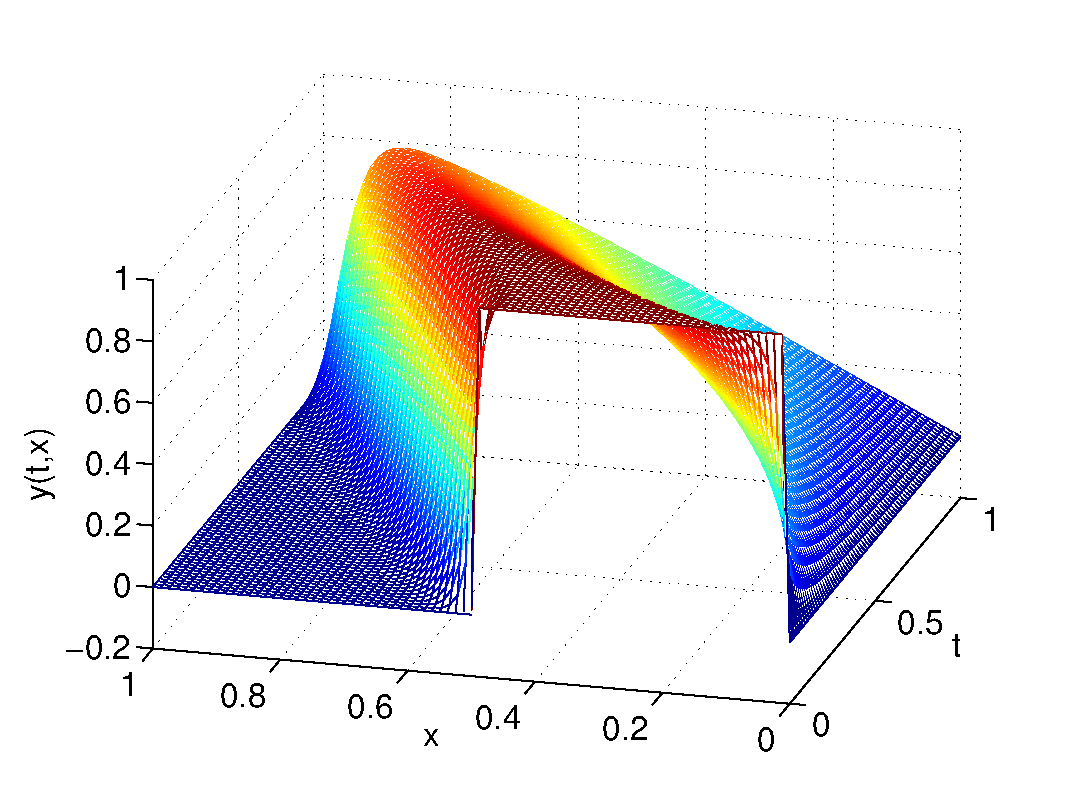
\includegraphics[width=0.49\textwidth]{plots/controlRedk1}}\hfill
\subfloat[$k=2$]{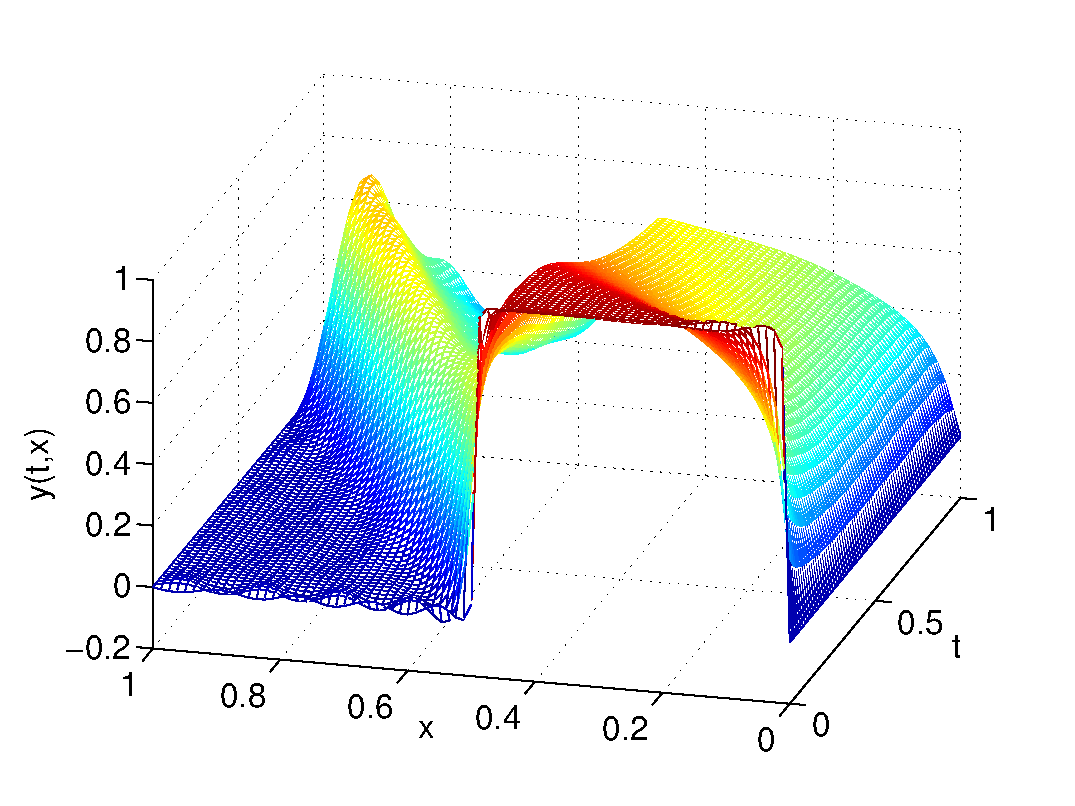
\includegraphics[width=0.49\textwidth]{plots/controlRedk2}}\\
\subfloat[$k=5$ ]{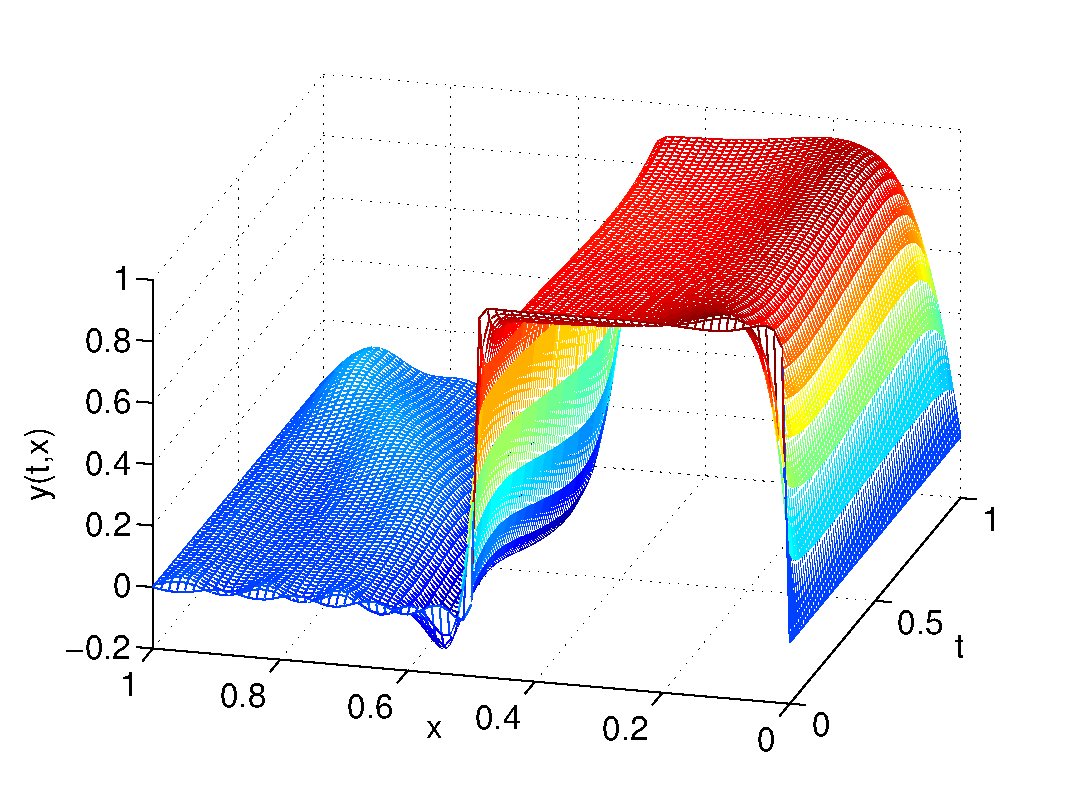
\includegraphics[width=0.49\textwidth]{plots/controlRedk5}}\hfill
\subfloat[$k=10$]{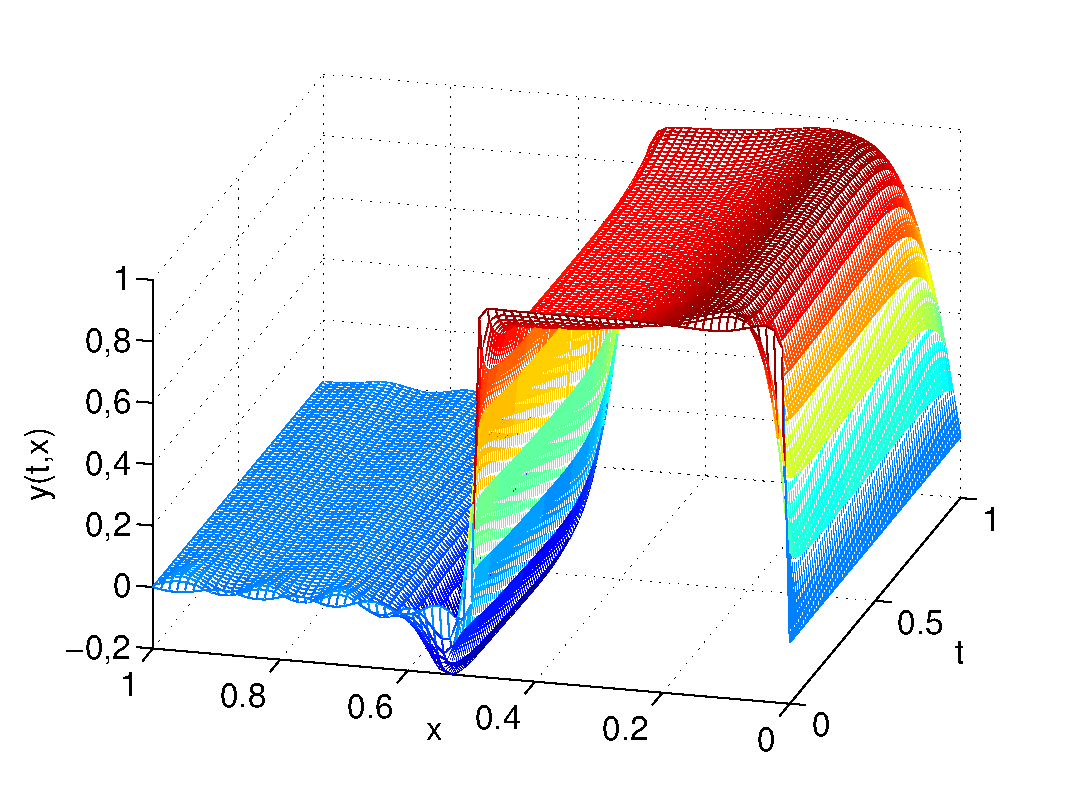
\includegraphics[width=0.49\textwidth]{plots/controlRedk10}}\\
\caption{Reduced-order optimization.}\label{optRed}
\end{figure}

\begin{figure}[H]
\centering
\subfloat[$k=1$ (initial)]{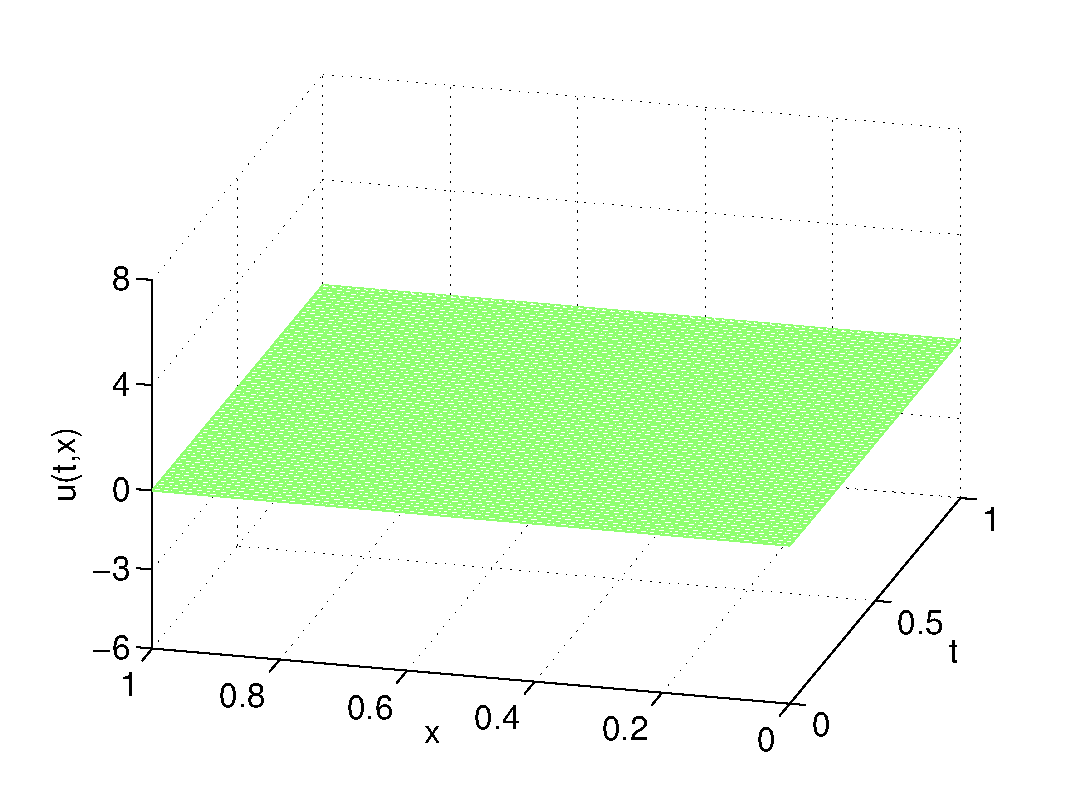
\includegraphics[width=0.49\textwidth]{plots/uRedk1}}\hfill
\subfloat[$k=2$]{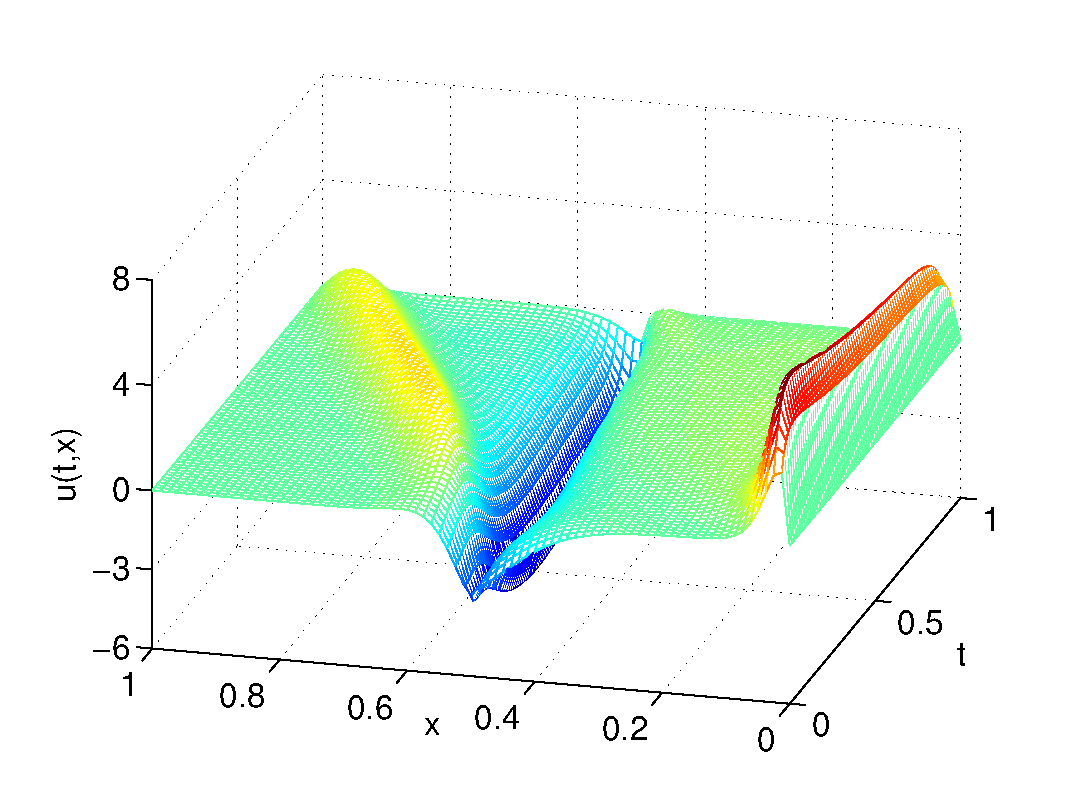
\includegraphics[width=0.49\textwidth]{plots/uRedk2}}\\
\subfloat[$k=5$ ]{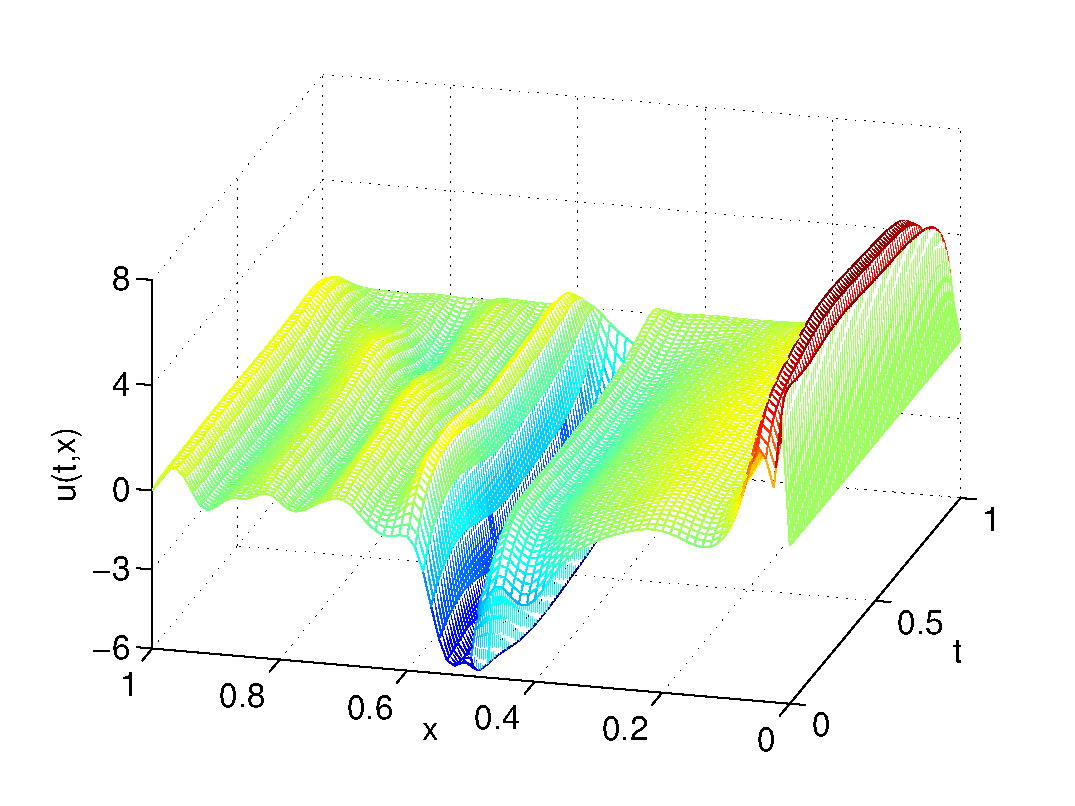
\includegraphics[width=0.49\textwidth]{plots/uRedk5}}\hfill
\subfloat[$k=10$]{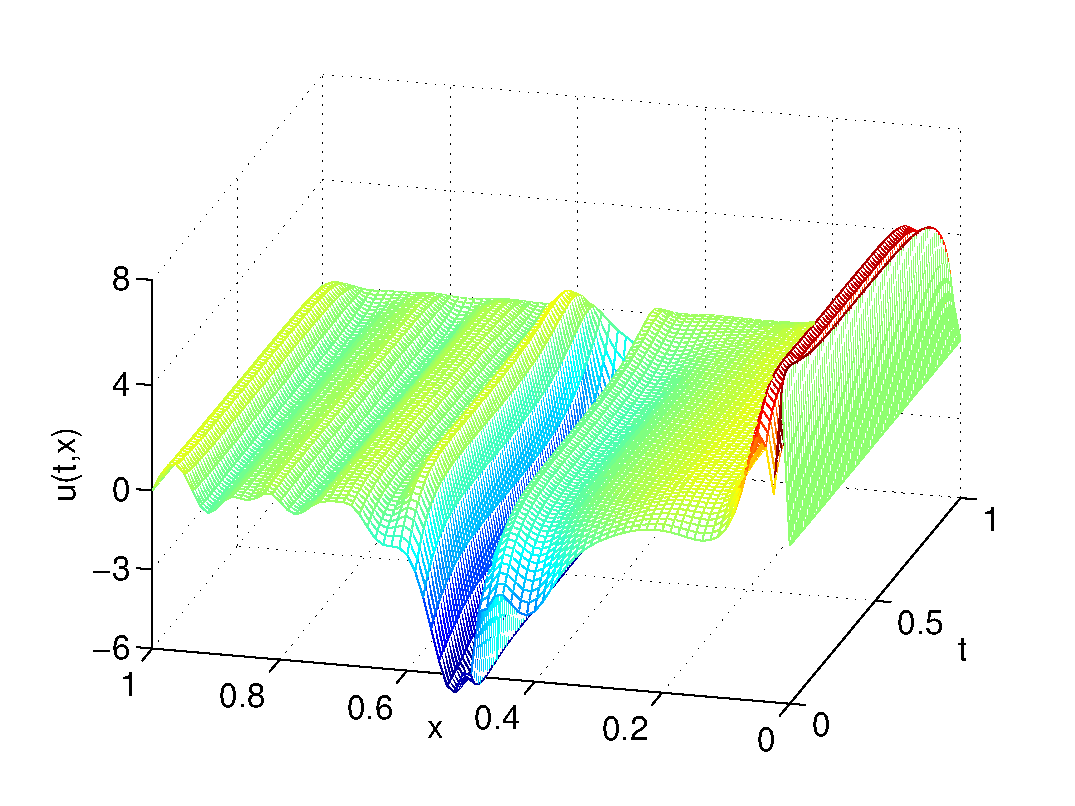
\includegraphics[width=0.49\textwidth]{plots/uRedk10}}\\
\caption{Reduced-order control.}\label{optRedu}
\end{figure}
%\section{Parameter study of the reduced model}
%\newpage
\section{Performance and error analysis}
For $\nu = 0.01$ full model $N = 80$. Chose DEIM-dimension constant, $m = 15$ and increase POD-dimension $\ell$ from $3$ to $25$. Interesting: for $\ell > m$, the error is dominated by the DEIM approximation error and does not decrease further...
\begin{figure}[H]
\centering
\subfloat{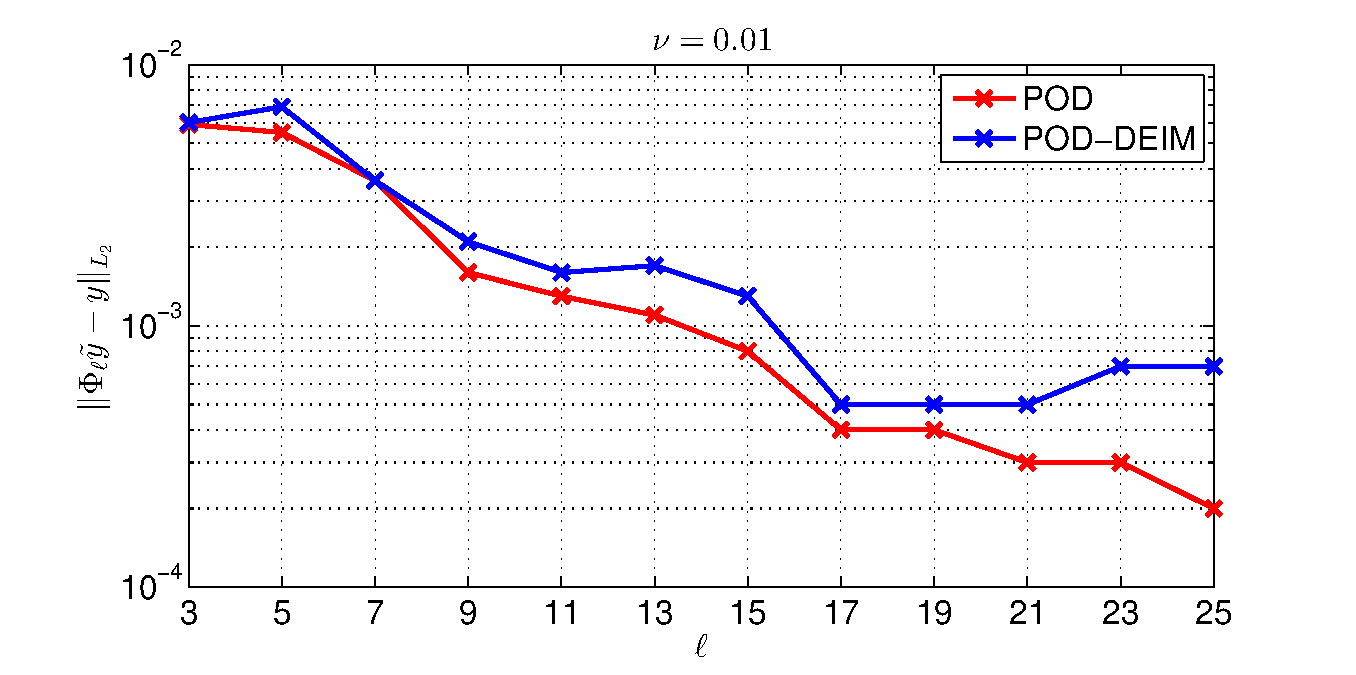
\includegraphics[width=0.7\textwidth]{plots/yL2err}}\\
\subfloat{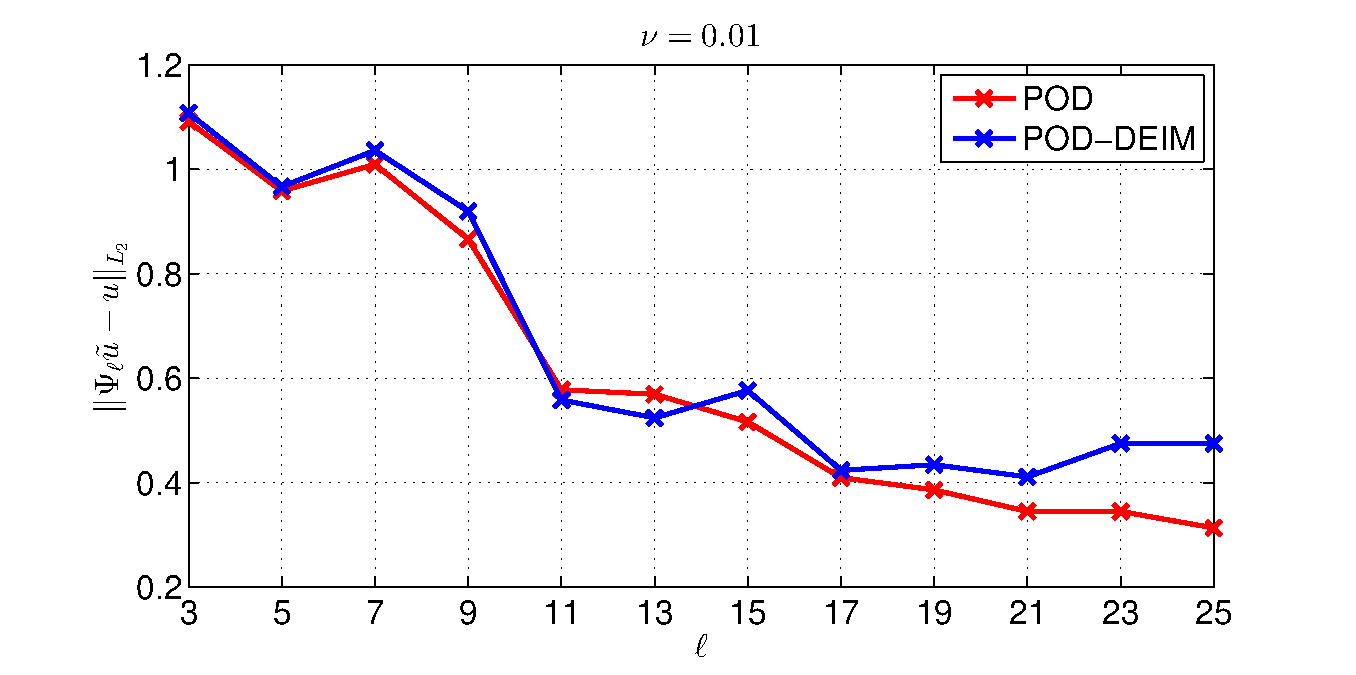
\includegraphics[width=0.7\textwidth]{plots/uL2err}}
\caption{Comparison of the $L_2$-error of the POD and the POD-DEIM approximation when the projection dimensions are increased.}\label{L2err}
\end{figure}

\begin{figure}[H]
\centering
\subfloat[$\ell = 5$]{\includegraphics[width=0.33\textwidth]{plots/YerrL2_pod_5}}\hfill
\subfloat[$\ell = 15$]{\includegraphics[width=0.33\textwidth]{plots/YerrL2_pod_15}}\hfill
\subfloat[$\ell = 25$]{\includegraphics[width=0.33\textwidth]{plots/YerrL2_pod_25}}\hfill \\
\subfloat[$\ell = 5$]{\includegraphics[width=0.33\textwidth]{plots/YerrL2_poddeim_5}}\hfill
\subfloat[$\ell = 15$]{\includegraphics[width=0.33\textwidth]{plots/YerrL2_poddeim_15}}\hfill
\subfloat[$\ell = 25$]{\includegraphics[width=0.33\textwidth]{plots/YerrL2_poddeim_25}}\hfill \\
\caption{Error in the $L_2$-norm compared between POD and POD-DEIM.}\label{YerrL2}
\end{figure}

\begin{table}[H]
\centering
\begin{tabular}{|c|c|c|c|c|c|c|c|c|c|}
\cline{1-10}
 & \multicolumn{3}{ c| }{Newton-type} & \multicolumn{3}{ c| }{BFGS}& \multicolumn{3}{ c| }{SPG}\\ \cline{2-10}
 & Full & POD & DEIM & Full & POD & DEIM & Full & POD & DEIM \\ \cline{1-10}
$N$/$\ell$/$m$ & $80$ &$ 11 $&$(11,13)$ & $200$&$35 $& $(35,40)$  & $800$&$40 $& $(40,55)$ \\ \cline{1-10}
$t_{setup}[s]$        & -      &0.003      &0.011       & -    &0.009&0.021 & -& 0.0729&0.182\\ \cline{1-10}
$t_{PDEsol}[s]$   &  0.068     &0.047      &0.040       & 0.232&0.12&0.055 & 4.416&0.276&0.085\\ \cline{1-10}
$e_{\ell,m}[10^{-4}]$   & -      &6.13       &6.46        & -    &6.12&6.85 & -&7.43& 7.66\\ \cline{1-10}
$S_P^{(1)}$           & -      &1.35       &1.34        & -    &1.74&3.03 & -&12.54&16.52\\ \cline{1-10}
$S_P^{(2)}$           & -      &1.44       &1.71        & -    &1.88&4.21 & -&15.85&51.85\\ \cline{1-10}
\end{tabular}
\caption{Time measurements for different optimization algorithms and $\nu = 0.01$.}\label{time_messure}
\end{table}
